\section{The Representation Layer: Clique Path Index} \label{sec:our_approach}

% 我们的算法的核心思想是通过对于每一个$r$-clique计算其$s$-clique的个数来进行计算, 无需枚举任何$s$-clique, 只需要知道数量即可. 
In this section, we present the representation layer of our method for nucleus decomposition, which addresses the limitations of existing methods by eliminating their reliance on explicit $s$-clique enumeration. 
%
The key idea of our algorithm is to leverage the proposed \textit{Clique Path Index} (\cpi) to directly count $s$-cliques while maintaining and updating the index dynamically during the peeling process. 
%
In the following, we first provide an overview of this counting/indexing layer, then review the background on clique counting, and finally present the definition and design of \cpi.


\subsection{Overview}
% \begin{algorithm}[t]
\small
% \caption{\textsc{$(r,s)$-CND}}
% \label{alg:framework}
% \KwIn{Clique size $s$}
% \KwOut{Core value $\kappa_s(v)$ for every vertex $v$}
% \SetKwFunction{RemoveNode}{RemoveNode}
% \SetKwFunction{CountPreEdges}{$s$-CliqueCount}
% \SetKwProg{Fn}{Function}{:}{}

% $\tree$ $\leftarrow$ build CPI of $G$, pruning paths with $s$\;

% $support \gets$ \textsc{CountPreEdges}$(\mathcal{B}, r, s)$\;

% build min heap $H_{\min}$ using $support$\;

% $c_{min} \gets 0$\;

% \While{$H_{\min}$ is not empty}{
%     $R_{min} \gets \text{ExtractMin}(H_{\min})$\;
%     $c_{min} \gets \max(c_{min}, support(R_{min}))$\;
%     $\kappa_s(R_{min}) \gets c_{min}$\;
%     \ForEach{leaf $\TPath$ intersecting any $rc \in R_{min}$}{
%         $B \gets {\,rc \in R_{min} \mid rc \in \TPath\,}$\;
%         \text{Remove all $r$-cliques in $B$ from $\TPath$}\;
%     }

%     \ForEach{leaf $\TPath$ containing any $rc \in R_{min}$}{
%         Update $support(rc)$ and $H_{\min}$ for all $r$-clique $rc \in \TPath$
%     }

% }

% \Return{$\kappa_s(r)$ for all $r$-cliques $r$ in $\tree$}\;

% \end{algorithm}

\begin{algorithm}[t]
\small
\caption{\textsc{$(r,s)$-\cbnd}}
\label{alg:framework}
\KwIn{Graph $G=(V,E)$, clique sizes $r<s$}
\KwOut{Core value $\kappa_s(R)$ for every $r$-clique $R$}
\SetKwFunction{RemoveNode}{RemoveNode}
\SetKwFunction{CountPreEdges}{$s$-CliqueCount}
\SetKwProg{Fn}{Function}{:}{}

$\tree \leftarrow \textsc{BuildIndex}(G)$\;

\tcp{initialize $s$-support for all $r$-cliques}

$support \gets$ \textsc{$s$-CliqueCount}$(\tree, r, s)$ 

build a min-heap $H_{\min}$ using $support$\;

$c_{min} \gets 0$\;

\While{$H_{\min}$ is not empty}{
    $R_{min} \gets \text{ExtractMin}(H_{\min})$\;
    $c_{min} \gets \max(c_{min}, support(R_{min}))$\;
    $\kappa_s(R_{min}) \gets c_{min}$\;
    
    % remove $R_{min}$ from index
    % Remove all $r$-cliques in $R_{min}$ from $\tree$\;
    \textsc{UpdateIndex}($R_{min}$, $\tree$) \tcp*{remove $R_{min}$ from $\tree$}

    \tcp{update support of affected $r$-cliques}

    \textsc{UpdateSupport}($R_{min}$, $\tree$, $support$, $H_{\min}$)

}

\Return{$\kappa_s(R)$ for all $r$-cliques $R$ in $\tree$}\;

\end{algorithm}

% 我们观察到, Nuclear Decomposition这个算法的输出只涉及到r-clique的coreness, 以及后续的hierarchy, 这些输出并不需要列举任何s-clique. s-clique仅仅是用来衡量r-clique的support, 因此我们认为避免显式的枚举s-clique是可行的. 
We observe that a key step in nucleus core decomposition is support computation.
%
For each $r$-clique, this step only needs the number of $s$-cliques that contain it.
%
This suggests that explicit enumeration of $s$-cliques is not necessary.
%
It is both feasible and desirable to avoid it.
Based on this observation, we propose a minimal counting-and-indexing layer, as shown in Algorithm~\ref{alg:framework}.



% 受此启发, 我们提出了一个最小化的基础框架, 如算法\ref{alg:framework}所示.
% 这个框架的关键在于通过索引来避免显式枚举s-clique, 具体来说有三个关键的操作需要索引来支持, 分别是: (i) 初始化每个r-clique的s-support(第2行), (ii) 删除已经peel掉的r-clique(第9行), 以及(iii) 精准识别和更新剩余受影响r-clique的support(第10行).
\stitle{Key Idea.} 
The core idea is simple.
%
We avoid explicit enumeration of $s$-cliques by using an auxiliary index. 
%
Our method still follows the peeling paradigm.
%
The index supports four key operations:
%
(i) \textsc{BuildIndex}, which initializes the auxiliary index structure (Line~1);  
(ii) \textsc{$s$-CliqueCount}, which computes the initial $s$-support for each $r$-clique (Line~2);  
(iii) \textsc{UpdateIndex}, which removes peeled $r$-cliques from the index (Line~9); and  
(iv) \textsc{UpdateSupport}, which identifies and updates the supports of affected $r$-cliques after each removal (Line~10).  
%
In the conference version, these four operations were mainly presented from a counting/indexing viewpoint.
%
In this journal version, operations (iii) and (iv) are lifted to the \emph{differential path contribution maintenance} view.
%
\textsc{UpdateIndex} only changes the local state of affected paths.
%
\textsc{UpdateSupport} uses exact differential updates of path contributions.
%
It does not use reconstructive support recomputation.
% 
\myaddRC{
Figure~\ref{fig:pipline} illustrates the overall pipeline of our approach.
}

\myaddRC{
\begin{figure}[t]
    \centering
    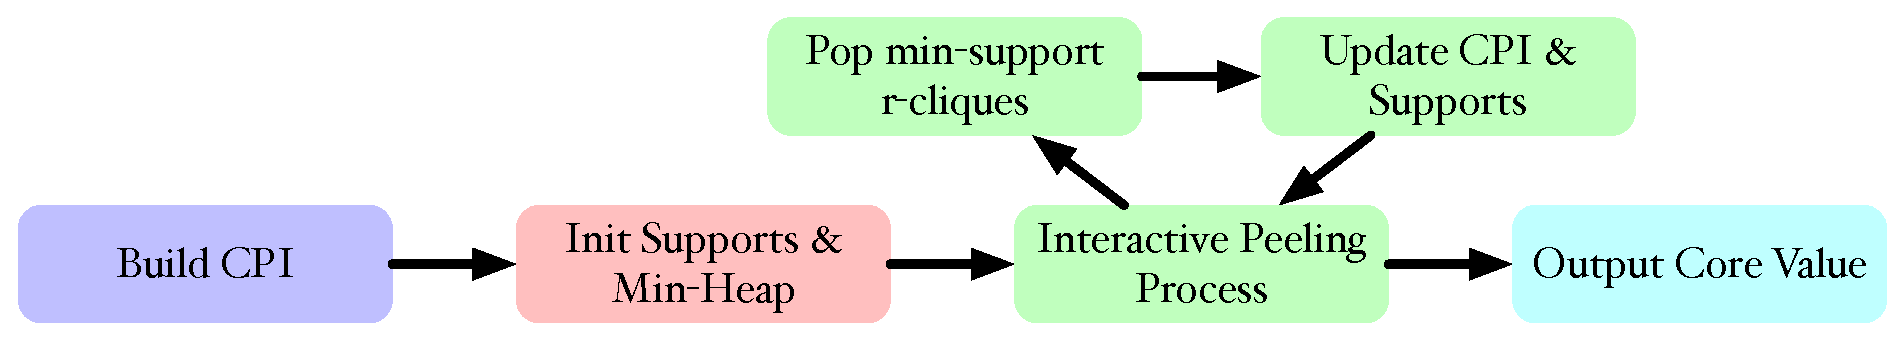
\includegraphics[width=0.45\textwidth]{figure/pipline.eps}
    % 虚线连接的节点是\pivot节点, 实线连接的节点是\hold节点.
    \caption{
        Overview of our approach.
    }
    \label{fig:pipline}
\end{figure}
}


\stitle{Index Support.}
% 上面说了4个
If an index supports these four operations efficiently, then nucleus decomposition can be performed without enumerating any $s$-cliques.
%
This removes the main bottleneck.
%
The key journal-level refinement is also simple.
%
The index is not only a compact representation of clique space.
%
It also carries the differential maintenance state used for exact support updates.
% 如果我们能找到一个索引来支持这三个操作, 那么我们就能在不枚举任何s-clique的情况下完成nuclear decomposition, 从而使算法变得不依赖于s-clique的枚举, 彻底摆脱枚举的瓶颈.


% Guided by this, we propose a minimal base framework: (i) build a CPI over $G$; (ii) compute the initial $s$-support for every $r$-clique; and (iii) peel in increasing support by repeatedly extracting the current minimum, assigning $\kappa_s(\cdot)$, removing the peeled $r$-cliques from CPI, and updating the supports of remaining neighbors along affected paths.

% To realize this framework \emph{without materializing $K_s$}, three lines in Algorithm~\ref{alg:hierarchy} require an index: line~2 (one-shot support initialization), line~11 (path-local removal of peeled $r$-cliques), and line~13 (incremental neighbor updates). Our goal is to carry out all three by \emph{counting} on CPI paths rather than \emph{enumerating} $s$-cliques.


% % \begin{algorithm}[htbp]
%     \caption{Bron-Kerbosch Algorithm}
%     \label{alg:bron_kerbosch}
%     \KwIn{Graph $G = (V, E)$}
%     \KwOut{All maximal cliques in $G$}
%     \SetKwFunction{FMain}{BronKerbosch}
%     \SetKwProg{Fn}{Function}{:}{}
%     \Fn{\FMain{$R, P, X$}}{
%         \If{$P = \emptyset \land X = \emptyset$}{
%             \Return $R$ \;
%         }
%         $u_{piv} \gets \arg\max_{x\in P} |P\cap N_H(x)|$ \;
%         \ForEach{$v \in P \setminus N(u_{piv})$}{
%             \FMain{$R \cup \{v\}, P \cap N(v), X \cap N(v)$} \;
%             $P \gets P \setminus \{v\}$ \;
%             $X \gets X \cup \{v\}$ \;
%         }
%     }
% \end{algorithm}

% \begin{algorithm}[htbp]
%     \caption{Bron-Kerbosch Algorithm}
%     \label{alg:bron_kerbosch}
%     \LinesNumbered
%     \KwIn{Undirected graph $G=(V,E)$}
%     \KwOut{All maximal cliques in $G$}
%     \SetKwFunction{BKMain}{BronKerbosch}
%     \SetKwProg{Fn}{Function}{:}{}

%     Compute a degeneracy ordering $(v_1,\dots,v_n)$ of $G$; let $\sigma(v_i)\leftarrow i$\;
%     Orient every edge from lower to higher rank to obtain $N^{+}(\cdot)$;
    
%     \ForEach{$v \in V$ in increasing order of $\sigma$}{
%         $P \gets N^{+}(v)$,\quad $X \gets N(v)\setminus N^{+}(v)$\;
%         \BKMain{$\{v\},\; P,\; X$}\;
%     }

%     \Fn{\BKMain{$R, P, X$}}{
%         \If{$P=\emptyset \land X=\emptyset$}{
%             \textbf{output clique }$R$\;
%             \Return
%         }
%         $u_{\text{piv}} \gets \arg\max_{x \in P \cup X} |\,P \cap N(x)\,|$ 
        
%         \ForEach{$v \in P \setminus N(u_{\text{piv}})$}{
%             \BKMain{$R \cup \{v\},\; P \cap N(v),\; X \cap N(v)$}\;
%             $P \gets P \setminus \{v\}$\;
%             $X \gets X \cup \{v\}$\;
%         }
%     }
    
    
% \end{algorithm}

% \begin{algorithm}[htbp]
%     \caption{Bron-Kerbosch Algorithm}
%     \label{alg:bron_kerbosch}
%     \KwIn{Graph $G=(V,E)$}
%     \KwOut{All maximal cliques in $G$ (each reported once)}
%     \SetKwFunction{BKMain}{BronKerbosch}
%     \SetKwProg{Fn}{Function}{:}{}

%     Compute a degeneracy ordering $(v_1,\dots,v_n)$ of $G$  
%     Orient every edge from lower to higher rank to obtain $N^{+}(\cdot)$\;

%     \ForEach{$v \in V$ in increasing order of $\sigma$}{
%         $P \gets N^{+}(v)$\;
%         \BKMain{$\{v\}, P$}\;
%     }

%     \Fn{\BKMain{$R, P$}}{
%         \If{$P=\emptyset$}{
%             \Return $R$ 
%         }
%         $u_{\text{piv}} \gets \arg\max_{x\in P} |P \cap N(x)|$ 

%         \ForEach{$v \in P \setminus N(u_{\text{piv}})$}{
%             \BKMain{$R \cup \{v\},\;\; P \cap N(v)$}\;
%             $P \gets P \setminus \{v\}$ 
%         }
%     }
    
% \end{algorithm}




% \begin{algorithm}[t!]
%     \caption{\textsc{Build--SCT}$(G,\,s)$}
%     \label{alg:buildSCT}
%     \KwIn{Undirected graph $G=(V,E)$, optional size cap $s$}
%     \KwOut{Succinct Clique Tree of $G$}

%     Compute a degeneracy ordering $(v_1,\dots,v_n)$ of $G$  
%     Orient every edge from lower to higher rank to obtain $N^{+}(\cdot)$\;

%     \For(\tcp*[f]{one root per vertex}){$i\gets 1$ \KwTo $n$}{
%         $V_{Hold}\gets\{v_i\}$ $P\gets N^{+}(v_i)$ $V_{Pivot}\gets\emptyset$

%         \textsc{ExpandPath}$(P, V_{Hold}, V_{Pivot})$\;
%     }

%     \SetKwFunction{Expand}{ExpandPath}
%     \SetKwProg{Fn}{Function}{:}{}

%     \Fn{\Expand{$P, V_{Hold}, V_{Pivot}$}}{
%         \If{$P=\emptyset$}{
%             \textbf{output path }$\{V_{Hold},\,V_{Pivot}\}$\;
%             \textbf{return}
%         }
        
%         $u_{piv} \gets \arg\max_{x\in P} |P\cap N^+(x)|$ \;
%         \For(\tcp*[f]{non-neighbors of pivot}){$v\in P\setminus N(u_{piv})$}{
%             $P\gets P\setminus\{v\}$
            
%             \eIf{$v=u_{piv}$}{
%                 \Expand{$P\cap N(v),\;V_{Hold},\;V_{Pivot}\cup\{v\}$}
%             }{
%                 \Expand{$P\cap N(v),\;V_{Hold}\cup\{v\},\;V_{Pivot}$}
%             }
%         }
%     }
% \end{algorithm}

% Lemma 4.6 (Path pruning). Let P be a path in the CPI and let
% 𝑠 ≥ 1 be the target clique size. Then P encodes at least one 𝑠-clique iff
% |𝑉ℎ (P)| ≤ 𝑠 ≤ |𝑉ℎ (P)| + |𝑉𝑝 (P)| .
% Equivalently, P can be safely pruned for size 𝑠 iff
% 𝑠 < |𝑉ℎ (P)| or 𝑠 > |𝑉ℎ (P)| + |𝑉𝑝 (P)| .
% Example 4.7. Considering the CPI shown in Figure 3, if we need

\begin{algorithm}[t!]
    \caption{\textsc{Build--CPI}$(G,\,s)$}
    \label{alg:buildCPI}
    \KwIn{Undirected graph $G=(V,E)$, optional size cap $s$}
    \KwOut{Clique Path Index (CPI) of $G$}

    Compute a degeneracy ordering $(v_1,\dots,v_n)$ of $G$  
    Orient every edge from lower to higher rank to obtain $N^{+}(\cdot)$\;

    \For(\tcp*[f]{one root per vertex}){$i\gets 1$ \KwTo $n$}{
        $V_{Hold}\gets\{v_i\}$ $P\gets N^{+}(v_i)$ $V_{Pivot}\gets\emptyset$

        \textsc{ExpandPath}$(P, V_{Hold}, V_{Pivot})$\;
    }

    \SetKwFunction{Expand}{ExpandPath}
    \SetKwProg{Fn}{Function}{:}{}

    \Fn{\Expand{$P, V_{Hold}, V_{Pivot}$}}{

    % path pruning
        \lIf{$|V_{Hold}| > s$}{
            \textbf{return}
        }

        \If{$P=\emptyset$}{
            %  \textbf{or} $|V_{Hold}| + |V_{Pivot}| < s
            % \textbf{output path }$\{V_{Hold},\,V_{Pivot}\}$\;
            % \textbf{return}
            \If{$|V_{Hold}| + |V_{Pivot}| \ge s$}{
                \textbf{output path }$\{V_{Hold},\,V_{Pivot}\}$\;
            }
            \textbf{return}
        }
        
        $u_{piv} \gets \arg\max_{x\in P} |P\cap N^+(x)|$ \;
        \For(\tcp*[f]{non-neighbors of pivot}){$v\in P\setminus N(u_{piv})$}{
            $P\gets P\setminus\{v\}$
            
            \eIf{$v=u_{piv}$}{
                \Expand{$P\cap N(v),\;V_{Hold},\;V_{Pivot}\cup\{v\}$}
            }{
                \Expand{$P\cap N(v),\;V_{Hold}\cup\{v\},\;V_{Pivot}$}
            }
        }
    }
\end{algorithm}

\subsection{Succinct Clique Tree} \label{sec:sct}

% \noindent\textit{Motivation from our base framework.}
% In the base framework (Algorithm~\ref{alg:hierarchy}, CND), three operations require an index that avoids materializing $K_s$: the one-shot initialization of $(r,s)$-supports (line 2), the path-local removal of peeled $r$-cliques (line 11), and the incremental update of neighbors' supports (line 13). Since the final output does not need to list any $s$-clique, we seek a counting representation rather than an enumeration of $K_s$.

% \noindent Succinct Clique Tree (SCT)\cite{Pivoter} is a Bron-Kerbosch-inspired representation that organizes the pivoting search space for exact clique counting.
% 
% \textit{Construction and stored semantics.} Using% \begin{definition}[clique path]
% \label{def:root_leaf_path}
% Given a \emph{Succinct Clique Tree}, a \emph{clique path}
% is a path that starts from the root node and ends at a leaf node, denoted as $\TPath{}$.
% All clique paths are enumerated in a \textbf{left-to-right
% depth-first search (DFS) order}.  We denote the $i$-th path in this
% DFS order by $\TPath{i}$.
%
% Formally, let
% \[
%   \TPath{i} = \langle v_{a_1}, v_{a_2}, \dots, v_{a_\ell} \rangle ,
% \]
% where $v_{a_1}$ is the root, $v_{a_\ell}$ is the corresponding leaf,
% and $\ell$ is the length of the path.  The index $i$ reflects the
% position of this path in the DFS enumeration described above.
% \end{definition}
%
% \begin{example}
% \label{ex:sct_example}
% Figure~\ref{fig:sct_example} shows an example of a Succinct Clique Tree
% (SCT). $\TPath{1} = \langle v_1, v_4, v_5, v_6 \rangle$, the second path is
% $\TPath{2} = \langle v_1, v_2, v_3, v_4, v_5 \rangle$. There are eleven
% clique paths in total, and the last path is $\TPath{11} = \langle v_8, v_9 \rangle$.
% \end{example}
%
%
% \begin{lemma}[Clique Count in a Path\cite{Pivoter}]
% \label{lem:clique_count}
% Let $\TPath{}$ be a clique path in an SCT, with
% $V_{p}(\TPath{})$ and $V_{h}(\TPath{})$ denoting its pivot
% and hold vertices, respectively.
% For any $k\ge |V_{h}(\TPath{})|$, every $k$-clique represented by
% $\TPath{}$ consists of all vertices in $V_{h}(\TPath{})$ and
% exactly $k-|V_{h}(\TPath{})|$ vertices chosen from $V_{p}(\TPath{})$.
% Hence $\#\text{$k$-cliques on }\TPath{}$ is equal to $ \binom{|V_{p}(\TPath{})|}{\,k-|V_{h}(\TPath{})|\,}.$
% \end{lemma}
%
% \begin{example}
%   For SCT as shown in Figure~\ref{fig:sct_example}.
%   $V_{p}(\TPath{1}) = \{v_4, v_5\}$ and
%   $V_{h}(\TPath{1}) = \{v_1,v_6\}$. Thus, the number of $3$-cliques on $\TPath{1}$ is equal to $ \binom{2}{\,3-2\,} = 2.$ $V_{p}(\TPath{2}) = \{v_2, v_3, v_4, v_5\}$ and $V_{h}(\TPath{2}) = \{v_1\}$. Thus, the number of $3$-cliques on $\TPath{2}$ is equal to $ \binom{4}{\,3-1\,} = 6.$
% \end{example} a degeneracy ordering, we orient edges from lower to higher rank to obtain $N^+(\cdot)$. For each vertex $v$ (in order), SCT starts a root with \emph{hold} set $V_h{=}\{v\}$ and \emph{pivot} set $V_p{=}N^+(v)$ and recursively expands by pivoting: choose a pivot $u\in V_p$ (e.g., maximizing $|V_p\cap N^+(u)|$) and branch only on $V_p\setminus N(u)$ while shrinking candidates to $V_p\cap N(\cdot)$. Each state stores exactly two sets—$V_h$ (already fixed) and $V_p$ (eligible extensions); along any path, $V_h$ are mandatory and $V_p$ are selectable, so a path summarizes a family of cliques without enumerating them one by one.

% \noindent\textit{SOTA counting in brief.}
% To efficiently count cliques without explicit enumeration, we first review the state-of-the-art clique counting method, the \textit{Succinct Clique Tree (\sct)}~\cite{Pivoter}. 
% \sct compacts the Bron--Kerbosch pivoting search space for exact clique counting. Vertices are processed in degeneracy order and edges are oriented to define $N^+(\cdot)$. For each root $v$, every state stores two sets—$V_h$ (hold, already fixed) and $V_p$ (pivot, eligible extensions). Pivoting on $u\in V_p$ branches only on $V_p\setminus N(u)$ while shrinking candidates to $V_p\cap N(\cdot)$. Thus each clique path succinctly summarizes a family of cliques without enumerating them.
We first review the state-of-the-art clique counting method, the \textit{Succinct Clique Tree} (\sct)~\cite{Pivoter}. 
The \sct compacts the Bron--Kerbosch pivoting search space for exact clique counting. 
Instead of enumerating all cliques, \sct constructs a hierarchical search tree in which each node corresponds to a state in the Bron--Kerbosch maximal clique search (the pivot-based version)~\cite{BronKerbosch,bitsetClique}, thereby implicitly representing all subcliques. 
Vertices are processed in \textit{degeneracy order}, and edges are oriented to define $N^+(\cdot)$. 
For each root vertex $v$ in \sct, every state maintains two sets: $V_h$ (\hold, already fixed) and $V_p$ (\pivot, eligible extensions). 
Pivoting on $u \in V_p$ branches only on $V_p \setminus N(u)$ while restricting candidates to $V_p \cap N(\cdot)$. 
Thus, each \textit{clique} path succinctly represents a family of cliques without enumerating them explicitly. 
This structure supports aggregated counting of all subcliques (of sizes $r$, $s$, etc.), enabling exact clique counting without enumeration.


% \begin{algorithm}[t]
\small
% \caption{UpdateSupport}
% \label{alg:updateSupport}
% % $R_{min}$, $I$, $support$, $H_{\min}$)
% \KwIn{$r$-cliques $R_{min}$ removed, \sct $I$, support map $support$, min heap $H_{\min}$}
% \KwOut{Updated support map $support$ and min heap $H_{\min}$}
% \SetKwFunction{UpdateIndex}{UpdateIndex}
% \SetKwProg{Fn}{Function}{:}{}

% \ForEach{path $\TPath$ in $I$ that intersects any $rc \in R_{min}$}{
%     \ForEach{$rc covered$ by $\TPath$}{
%         old$\gets support(rc)$\;
%         recompute $support(rc)$ based on $\TPath$\;
%         \If{support(rc) changed}{
%             update $H_{\min}$ with new support value\;
%         }
%     }
% }
% \end{algorithm}

% 
% Bron-Kerbosch\cite{BronKerbosch}是枚举极大团的经典算法, 其通过对三个顶点集合$R$, $P$, $X$的递归回溯来枚举所有极大团. 其中$R$表示当前已经找到的极大团, $P$表示当前可能的顶点集合, $X$表示已经被排除的顶点集合. 该算法的时间复杂度为$O(3^{n/3})$, 其中$n$是图中顶点的个数.
% \paragraph{Bron--Kerbosch enumeration framework.}

% During each recursive call it keeps three pairwise-disjoint vertex sets, 
% $R$ denotes the current (partial) clique,
% $P$ comprises those vertices that may still be added to extend $R$,
% and $X$ collects vertices that have already been explored and must therefore be excluded.
% Given a vertex $v\in P$, the algorithm moves $v$ into $R$, updates
% $P\leftarrow P\cap N(v)$ and $X\leftarrow X\cap N(v)$, and then recurses.
% When both $P$ and $X$ become empty, $R$ constitutes a maximal clique.
% 首先先把图中的定点按照退化序进行排序,随后按照退化许序进行枚举. 每次只关注ordering中比当前顶点大的邻居, 这样可以避免重复枚举.
% 随后在\BKMain中, 如果$P$为空, 则说明当前的$R$是一个极大团, 将其输出. 否则选择一个枢纽顶点$u_{piv}$, 只对$P\setminus N(u_{piv})$中的顶点进行递归. 这样可以大大减少递归的分支数.
% At line 1, the algorithm first computes a degeneracy ordering of the graph and orients every edge from lower to higher rank to obtain $N^{+}(\cdot)$. Then, it iterates over each vertex $v$ in increasing order of the degeneracy ordering $\sigma$ at line 3. For each vertex $v$, it initializes the candidate set $P$ to $N^{+}(v)$ and calls the recursive function \BKMain with the current clique $R$ initialized to $\{v\}$ and the candidate set $P$ at line 4.

% In the recursive function \BKMain, if the candidate set $P$ is empty, it indicates that the current clique $R$ is maximal, and it is output at line 7. Otherwise, a pivot vertex $u_{\text{piv}}$ is selected at line 9, and the algorithm recurses only on the vertices in $P\setminus N(u_{\text{piv}})$ at line 11. This strategy significantly reduces the number of recursive branches.

% \begin{figure*}[htbp]
%     \centering
%     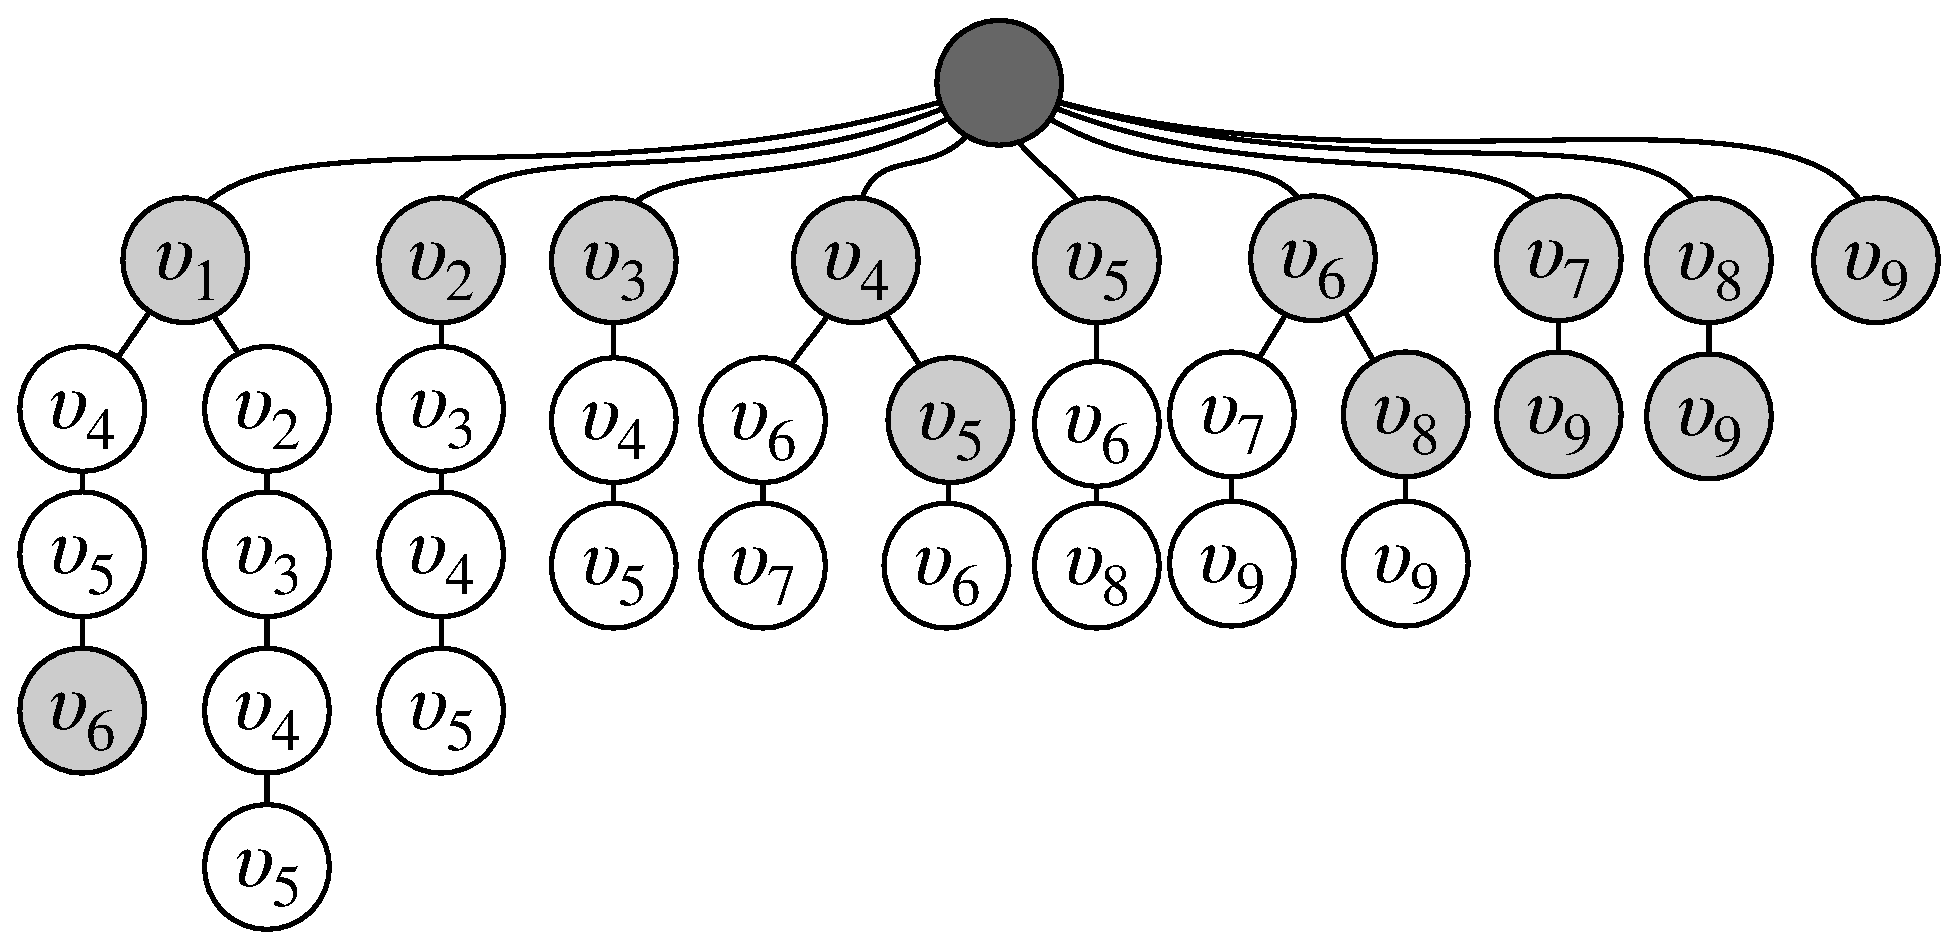
\includegraphics[width=0.9\textwidth]{figure/tree.eps}
%     \caption{An example of a Succinct Clique Tree (SCT). The white nodes represent pivots.}
%     \label{fig:sct_example}
% \end{figure*}
\begin{figure}[tb]
    \centering
    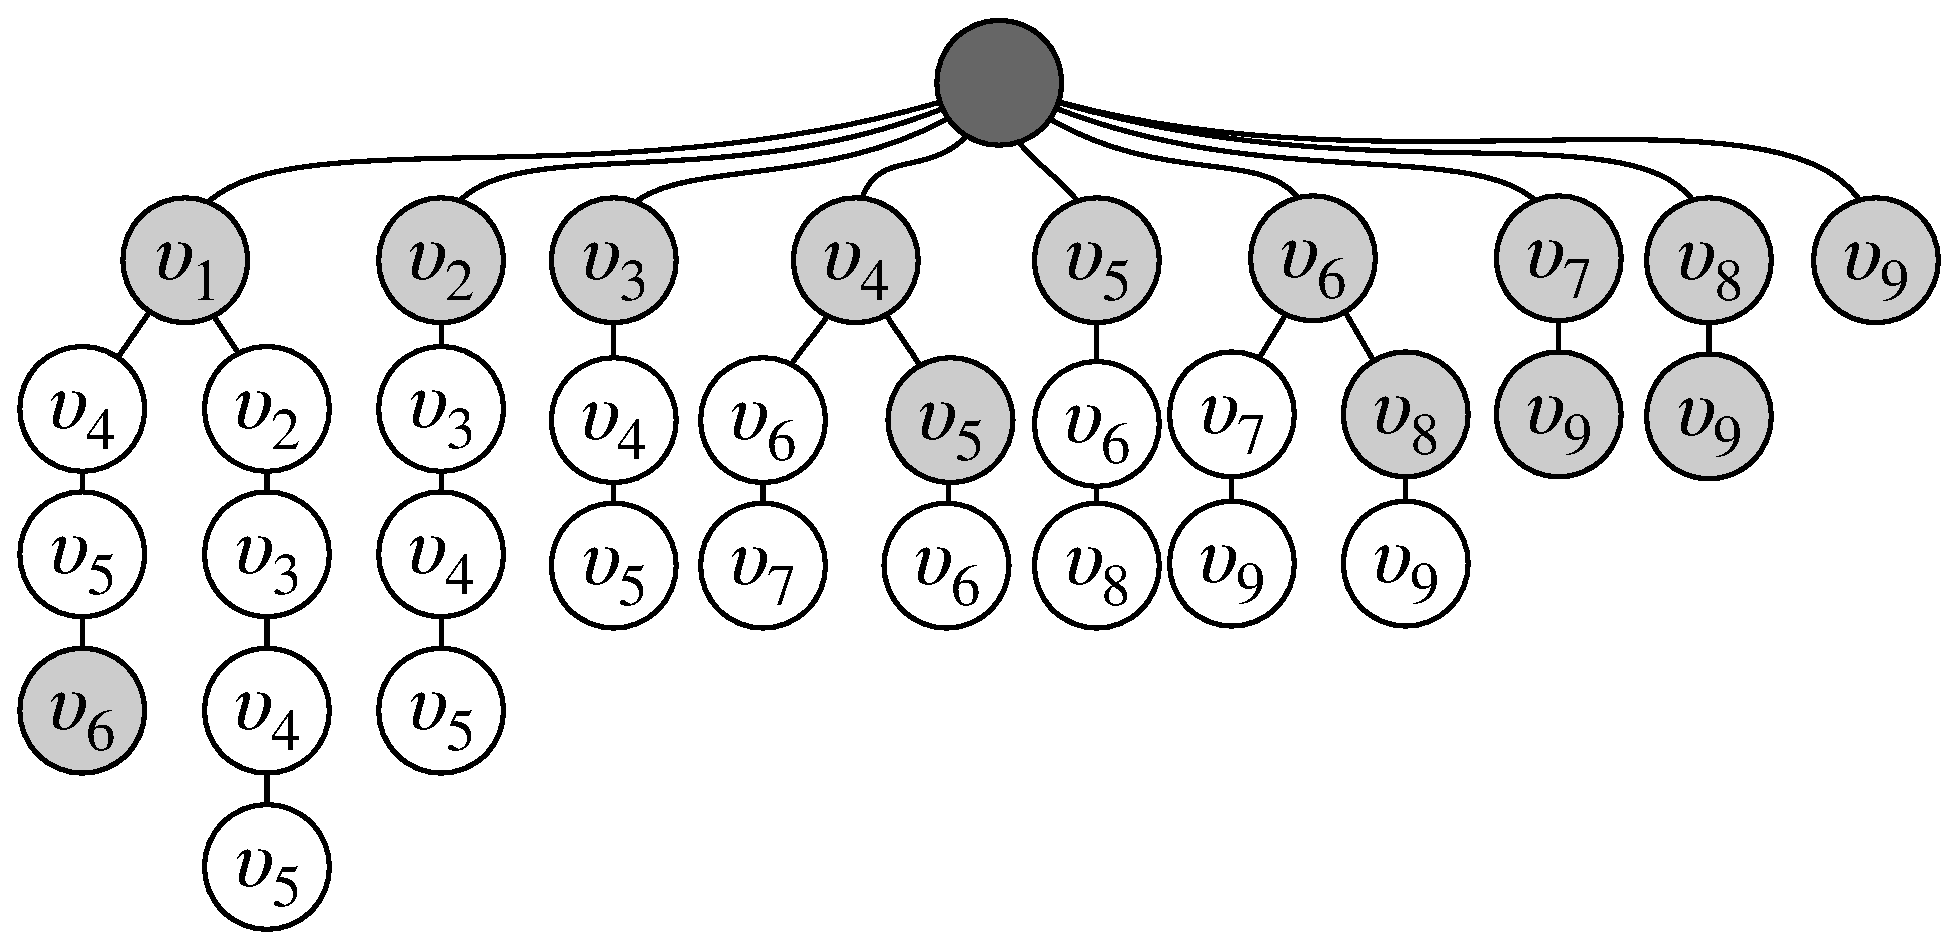
\includegraphics[width=0.43\textwidth]{figure/tree.eps}
    \caption{An example of a Succinct Clique Tree (\sct). White nodes denote pivots; gray nodes denote holds.}
    \label{fig:sct_example}
\end{figure}

% 基于出名的Bron-Kerbosch的理论, \cite{Pivoter}对此进行了一些改进, 提出了一个基于压缩的Succinct Clique Tree (SCT)的表示方法. 他们删除了$X$集合, 只保留$R$和$P$两个集合, 如Algorithm~\ref{alg:buildSCT}所示.
% The Bron--Kerbosch algorithm\cite{BronKerbosch,bitsetClique} is a seminal backtracking scheme for enumerating maximal cliques. Building on the same pivoting-style search space, Pivoter\cite{Pivoter} introduced the Succinct Clique Tree (SCT), which organizes the recursion into a compact multiway structure. Each state carries two sets: a \emph{hold} set $V_h$ (vertices already selected) and a \emph{pivot} set $V_p$ (eligible extensions), compactly capturing families of cliques. Figure~\ref{fig:sct_example} shows the SCT constructed for the example graph in Figure~\ref{fig:graph_example}.

% The Bron-Kerbosch algorithm\cite{BronKerbosch,bitsetClique} is a seminal back-tracking scheme for enumerating all maximal cliques in an undirected graph. 
% Based on the Bron-Kerbosch algorithm, \cite{Pivoter} introduced a Succinct Clique Tree (SCT) representation method that compresses the search space, as shown in Algorithm~\ref{alg:buildSCT}. The algorithm ultimately generates a multi-way tree, where each clique path represents a clique.
Figure~\ref{fig:sct_example} illustrates the SCT constructed for the example graph shown in Figure~\ref{fig:graph_example}.
% 为了方便后续介绍, 我们定义了根到叶子的路径, 如下所示:
We first define a \textit{clique path} as follows: 


\begin{definition}[Clique Path]\label{def:root_leaf_path}
In a Succinct Clique Tree, a \emph{clique path} $\TPath{}$ is any root-to-leaf path.  
All clique paths are enumerated in left-to-right depth-first order, with the $i$-th path denoted by $\TPath{i}$.
Formally,
$
  \TPath{i} = \langle v_{a_1}, v_{a_2}, \dots, v_{a_\ell} \rangle,
$
where $v_{a_1}$ is the root, $v_{a_\ell}$ is the leaf, and $\ell$ is the path length.
\end{definition}


\begin{example}
\label{ex:sct_example}
Figure~\ref{fig:sct_example} shows an example of a \sct. $\TPath{1} = \langle v_1, v_4, v_5, v_6 \rangle$, the second path is
$\TPath{2} = \langle v_1, v_2, v_3, v_4, v_5 \rangle$. There are eleven
clique paths in total, and the last path is $\TPath{11} = \langle v_8, v_9 \rangle$.
\end{example}


% \begin{lemma}[Clique Count in a Path~\cite{Pivoter}]
\begin{lemma}[Unique Path Encoding~\cite{Pivoter}]
\label{lem:clique_count}
% Let $\TPath{}$ be a clique path in an \sct, with
% $V_{p}(\TPath{})$ and $V_{h}(\TPath{})$ denoting its pivot
% and hold vertices, respectively.
% For any $k\ge |V_{h}(\TPath{})|$, every $k$-clique represented by
% $\TPath{}$ consists of all vertices in $V_{h}(\TPath{})$ and
% exactly $k-|V_{h}(\TPath{})|$ vertices chosen from $V_{p}(\TPath{})$.
% Hence $\#\text{$k$-cliques on }\TPath{}$ is equal to $ \binom{|V_{p}(\TPath{})|}{\,k-|V_{h}(\TPath{})|\,}.$

% 对于图中任何的$k$-clique $C_k$, 都存在且仅存在一个根到叶子的路径$\TPath{} = V_h(\TPath{}) \cup V_p(\TPath{})$满足$V_h(\TPath{}) \subseteq C_k \subseteq V_h(\TPath{}) \cup V_p(\TPath{})$. 其中$V_h(\TPath{})$和$V_p(\TPath{})$分别表示路径$\TPath{}$上的hold顶点和pivot顶点集合.
For any $k$-clique $C_k$ in the graph, there exists only one clique path $\TPath{} = V_h(\TPath{}) \cup V_p(\TPath{})$ such that $V_h(\TPath{}) \subseteq C_k \subseteq (V_h(\TPath{}) \cup V_p(\TPath{}))$. Here, $V_h(\TPath{})$ and $V_p(\TPath{})$ denote the sets of hold vertices and pivot vertices on the path $\TPath{}$, respectively.
\end{lemma}

Intuitively, any $k$-clique represented by a path $\TPath$ must include all hold vertices of that path, while the pivot vertices are optional. 
%
Formally, a $k$-clique $C_k$ is \emph{encoded} by a \cpi\ path $\TPath$ if and only if $V_h(\TPath) \subseteq C_k \subseteq V_h(\TPath) \cup V_p(\TPath)$; 
it is \emph{covered} by $\TPath$ if and only if  $C_k \subseteq V_h(\TPath) \cup V_p(\TPath)$.


\begin{example}
  For \sct as shown in Figure~\ref{fig:sct_example}.
  $V_{p}(\TPath{1}) = \{v_4, v_5\}$ and
  $V_{h}(\TPath{1}) = \{v_1,v_6\}$. Thus, the number of $3$-cliques on $\TPath{1}$ is equal to $ \binom{2}{\,3-2\,} = 2.$ $V_{p}(\TPath{2}) = \{v_2, v_3, v_4, v_5\}$ and $V_{h}(\TPath{2}) = \{v_1\}$. Thus, the number of $3$-cliques on $\TPath{2}$ is equal to $ \binom{4}{\,3-1\,} = 6.$
\end{example}

% \noindent\textit{Scope.}

\stitle{Inadequacies in \sct Structures.} 
\sct is designed solely for clique counting on static graphs. 
For the key functions in our framework (Algorithm~\ref{alg:framework}), 
\sct can support \textsc{$s$-CliqueCount} (i.e., initializing the support) with minor modifications. 
However, it lacks dynamic update capabilities and cannot be trivially extended to support \textsc{UpdateIndex} and \textsc{UpdateSupport}, which are required in our representation layer to remove peeled $r$-cliques efficiently. 
%
This limitation motivates the design of a new index that can support all these operations, which is both non-trivial and challenging.


% our Clique Path Index (\cpi) in next subsection, which adapts SCT to support efficient batched updates.
% a static counting structure: it directly supports 
% line~2 (one-shot initialization of $(r,s)$-supports) 
% but does not provide the dynamic path-local updates required by line~9 (removing peeled $r$-cliques from the index) and line~10 (updating neighbors' supports). 
% This limitation motivates our Clique Path Index (\cpi) in next subsection, which adapts SCT to support efficient batched updates.


% (i) \textsc{$s$-CliqueCount}, which initializes the $s$-support for each $r$-clique (Line~2); 
% (ii) \textsc{UpdateIndex}, which removes peeled $r$-cliques (Line~9); and 
% (iii) \textsc{UpdateSupport}, which identifies and updates the supports of affected $r$-cliques after each removal (Line~10). 

\subsection{Clique Path Index}
\label{sec:cpi}

% 在介绍我们的Derivation之前, 我们需要介绍一些基于SCT的概念和定理. 这些定理和概念是我们算法的基础.
% Before introducing our derivations, we need to present some \sct-based concepts and theorems that form the foundation of our algorithm.

% \begin{definition}[Clique path]
% \label{def:root_leaf_path}
% Given a \emph{Succinct Clique Tree}, a \emph{clique path}
% is a path that starts from the root node and ends at a leaf node, denoted as $\TPath{}$.
% All clique paths are enumerated in a \textbf{left-to-right
% depth-first search (DFS) order}.  We denote the $i$-th path in this
% DFS order by $\TPath{i}$.

% Formally, let
% \[
%   \TPath{i} = \langle v_{a_1}, v_{a_2}, \dots, v_{a_\ell} \rangle ,
% \]
% where $v_{a_1}$ is the root, $v_{a_\ell}$ is the corresponding leaf,
% and $\ell$ is the length of the path.  The index $i$ reflects the
% position of this path in the DFS enumeration described above.
% \end{definition}

% \begin{example}
% \label{ex:sct_example}
% Figure~\ref{fig:sct_example} shows an example of a Succinct Clique Tree
% (\sct). $\TPath{1} = \langle v_1, v_4, v_5, v_6 \rangle$, the second path is
% $\TPath{2} = \langle v_1, v_2, v_3, v_4, v_5 \rangle$. There are eleven
% clique paths in total, and the last path is $\TPath{11} = \langle v_8, v_9 \rangle$.
% \end{example}


% \begin{lemma}[Clique Count in a Path\cite{Pivoter}]
% \label{lem:clique_count}
% Let $\TPath{}$ be a clique path in an \sct, with
% $V_{p}(\TPath{})$ and $V_{h}(\TPath{})$ denoting its pivot
% and hold vertices, respectively.
% For any $k\ge |V_{h}(\TPath{})|$, every $k$-clique represented by
% $\TPath{}$ consists of all vertices in $V_{h}(\TPath{})$ and
% exactly $k-|V_{h}(\TPath{})|$ vertices chosen from $V_{p}(\TPath{})$.
% Hence $\#\text{$k$-cliques on }\TPath{}$ is equal to $ \binom{|V_{p}(\TPath{})|}{\,k-|V_{h}(\TPath{})|\,}.$
% \end{lemma}

% \begin{example}
%   For \sct as shown in Figure~\ref{fig:sct_example}.
%   $V_{p}(\TPath{1}) = \{v_4, v_5\}$ and
%   $V_{h}(\TPath{1}) = \{v_1,v_6\}$. Thus, the number of $3$-cliques on $\TPath{1}$ is equal to $ \binom{2}{\,3-2\,} = 2.$ $V_{p}(\TPath{2}) = \{v_2, v_3, v_4, v_5\}$ and $V_{h}(\TPath{2}) = \{v_1\}$. Thus, the number of $3$-cliques on $\TPath{2}$ is equal to $ \binom{4}{\,3-1\,} = 6.$
% \end{example}

Building on the basic idea of \sct~\cite{Pivoter}, we introduce a new data structure, the \emph{Clique Path Index} (\cpi), which is adapted to our counting-and-peeling framework and supports efficient updates.
% 
Unlike \sct, \cpi\ represents the search space as independent paths in a bipartite-like layout between vertices and paths, as illustrated in Figure~\ref{fig:new_tree_example}.
%
Thanks to this bipartite-like storage structure, we can also efficiently retrieve the paths containing each vertex and the vertices contained in each path, facilitating the implementation of the $\textsc{UpdateSupport}$ function in our framework to accurately identify affected $r$-cliques. 
% \cpi\ can be updated more efficiently than a traditional tree structure, as discussed in the next section.
Updating a traditional tree is difficult, since shared prefixes cause cascaded changes and costly subtree reattachments; accordingly, \cpi\ admits more efficient updates (details in the next section).


\begin{example}
    Figure~\ref{fig:new_tree_example} shows an example of a \cpi consisting of three paths and five vertices.
    Path 1 contains vertices $v_1,v_2,v_3,v_4,v_5$, where $v_1$ is a hold vertex and the others are pivot vertices.
    Path 2 contains vertices $v_1,v_4,v_5,v_6$, where $v_1$ and $v_6$ are hold vertices and the others are pivot vertices.
    Path 3 contains vertices $v_2,v_3,v_4,v_5$, where $v_2$ is a hold vertex and the others are pivot vertices.
\end{example}
% 

\begin{figure}[t]
  \centering
  \begin{subfigure}[t]{0.48\linewidth}
    \centering
    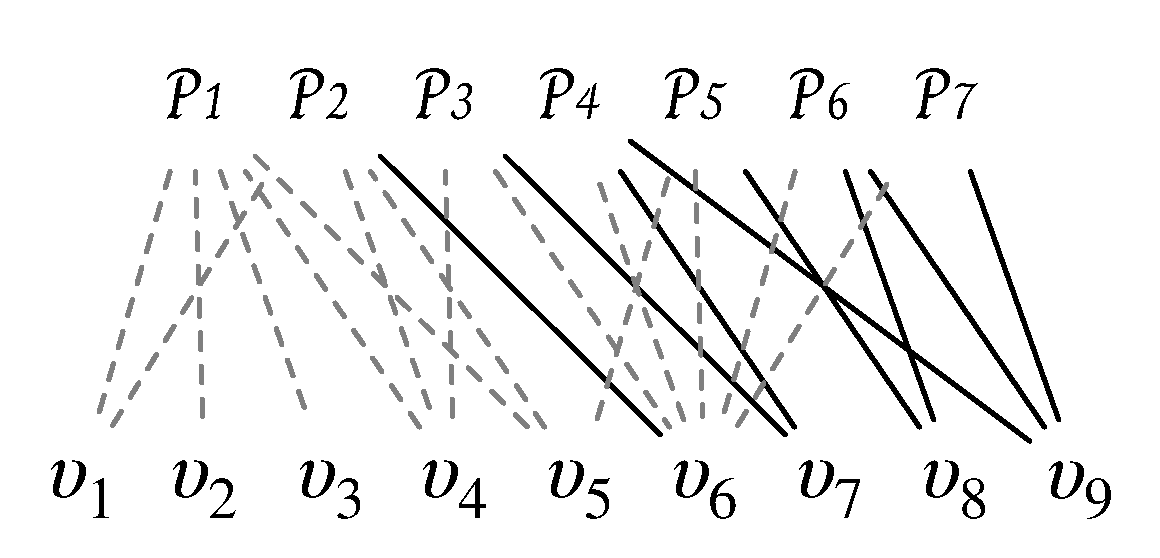
\includegraphics[width=0.8\linewidth]{figure/CPIlarge.eps}
    \caption{An example of a \cpi on Figure~\ref{fig:graph_example} (no pruning).}
    \label{fig:new_tree_example}
  \end{subfigure}
  \hspace{0.01\linewidth}
  \begin{subfigure}[t]{0.48\linewidth}
    \centering
    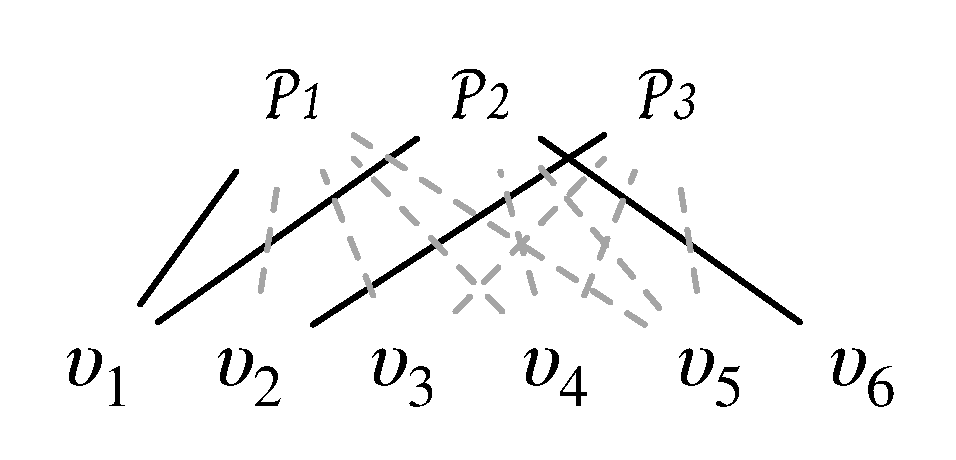
\includegraphics[width=0.8\linewidth]{figure/pruningTree.eps}
    \caption{An example of a pruned \cpi\ for $s=4$ on Figure~\ref{fig:sct_example}.}
    \label{fig:pruning_example}
  \end{subfigure}

  \caption{Examples of \cpi\ before and after pruning. Dashed nodes denote pivots, and solid nodes denote holds.}
\end{figure}

% 这种存储格式还使得我们可以高效获取到每个点所在的path以及每个path包含的点, 这使得我们可以完成我们Framework中$\textsc{UpdateSupport}$, 帮助我门来准确识别受影响的$r$-clique.
% This storage format also enables efficient retrieval of the paths containing each vertex and the vertices contained in each path, facilitating the implementation of the $\textsc{UpdateSupport}$ function in our framework to accurately identify affected $r$-cliques.



% \paragraph{Path-index storage (\cpi).}
% % 为了让tree可以高效的进行更新, 因此我们使用了二部图的方法来存储这个index, 具体来说, 我们分别存储每一条路径的hold节点和pivot节点, 如图\ref{fig:new_tree_example}所示.
% To enable efficient updates to the tree, we store the index using a bipartite-like approach. Specifically, we store the hold and pivot vertices of each path separately, 
% 该图中有

% 这里应该有\cpi的formal definition, 以及和SCT的区别.
% \todo{}


% To facilitate our discussion, We use two path-clique relations. A k-clique $C_k$ is covered by a CPI path \(\TPath\) if all its vertices lie on the path, i.e., \(C_k \subseteq V_h(\TPath)\cup V_p(\TPath)\). It is encoded by \(\TPath\) if, in addition, the path’s holds are mandatory: \(V_h(\TPath)\subseteq C_k \subseteq V_h(\TPath)\cup V_p(\TPath)\). Hence encoding implies coverage; conversely, a covered clique is encoded exactly when it contains all holds.

% To facilitate the discussion, we define that a $k$-clique $C_k$ is \emph{encoded} by a \cpi\ path $\TPath$ if and only if $V_h(\TPath) \subseteq C_k \subseteq V_h(\TPath) \cup V_p(\TPath)$. 
%
% Similarly, we define that a $k$-clique $C_k$ is \emph{covered} by a \cpi\ path $\TPath$ if and only if $C_k \subseteq V_h(\TPath) \cup V_p(\TPath)$.




% we define two types of relationships between a clique and a \cpi path based on the above theorem.

% \begin{definition}[Coverage of a $k$-clique by a path]
% \label{def:coverage_on_path}
% Let $\TPath{}$ be a CPI path with vertex set $V_h(\TPath{})\cup V_p(\TPath{})$.
% Given a $k$-clique $C_k$, we say that $C_k$ is \emph{covered} by $\TPath{}$ if and only if
% $C_k \subseteq V_h(\TPath{}) \cup V_p(\TPath{})$.
% \end{definition}


% \begin{definition}[Encoding of a $k$-clique by a path]
% \label{def:encoded_by}
% Let $\TPath{}$ be a CPI path with hold/pivot sets $V_h(\TPath{}),V_p(\TPath{})$.
% Given a $k$-clique $C_k$, we say that $C_k$ is \emph{encoded} by $\TPath{}$ if and only if
% $V_h(\TPath{}) \subseteq C_k \subseteq V_h(\TPath{}) \cup V_p(\TPath{})$.
% \end{definition}



Based on Lemma~\ref{lem:clique_count}, we derive Lemma~\ref{lem:s_support_r}, which enables the computation of the number of $s$-cliques for each $r$-clique without enumerating any $s$-cliques.

\begin{lemma}[Local $s$-support of an $r$-clique]
\label{lem:s_support_r}
Let $\TPath{}$ be a path in the \cpi with
pivot set $V_{p}$ and hold set $V_{h}$
$(h=|V_{h}|,\;p=|V_{p}|)$,
and fix integers $0<r<s$.
For any $r$-clique $C_r\subseteq\TPath{}$ set
$b \;=\; |\,C_r\cap V_{p}\,|,$
Then the number of distinct $s$-cliques on $\TPath{}$ that contain
$C_r$ equals
$
\#_{s}(C_r)
\;=\;
\binom{p-b}{\,s-h-b}.
$
\end{lemma}

\begin{proof}
Every $s$-clique on the path is
$V_h\cup Q$ with $Q\subseteq V_p$ and $|Q|=s-h$
(Lemma \ref{lem:clique_count}).
Fix any $r$-clique $C_r$ and let $b=|C_r\cap V_p|$.
Since $C_r$ already contributes those $b$ pivots,
an $s$-clique containing $C_r$ is obtained precisely by choosing the
remaining $s-h-b$ pivots from the $p-b$ unused pivots in $V_p$.
The number of such choices is
$\binom{p-b}{\,s-h-b}$,
which is zero whenever the lower or upper bound is violated.
\end{proof}
% 基于Lemma~\ref{lem:clique_count}, 我们可以在不枚举任何$s$-clique的情况下计算每个$r$-clique的$s$-clique的个数.同时考虑到我们只需要考虑$s$-clique的数量, 我们可以对SCT进行一些优化, 忽视掉那些不包含$r$-clique的路径.
% Based on Lemma~\ref{lem:clique_count}, we can compute the number of $s$-cliques for each $r$-clique without enumerating any $s$-cliques, as shown in Algorithm~\ref{alg:local_s_clique_count}. 

% 
% 基于Lemma~\ref{lem:s_support_r}, 我们推出了算法~\ref{alg:local_s_clique_count}. 来计算每个$r$-clique的$s$-clique的个数.
% \Fn{CountPreClique}{
%     \KwIn{SCT $\tree$, Clique size $r$, Clique size $s$}
%     \KwOut{$s$-clique count for every $r$-clique in $\tree$}
%     initialise $count(C_r)\leftarrow 0$ for all $r$-cliques in $\tree$\;
%     \ForEach{clique path $\TPath{}$ in $\tree$}{
%         \ForEach{$r$-clique $C_r$ in $\TPath{}$}{
%             % let $P$ be the set of pivots and $H$ be the set of holds along $\TPath{}$\;
%             $V_{p}\gets \{v \in \TPath{} \mid v \text{ is a pivot}\}$;

%             $V_{h}\gets \{v \in \TPath{} \mid v \text{ is a hold}\}$

%             $need\gets s-|V_{h}|$\;
%             $count(C_r)\gets count(C_r)+\binom{|V_{p}|}{need}$ for every $C_r\in \TPath{}$\;
%         }
%     }

%     \Return $count(C_r)$ for all $r$-cliques in $\tree$; 
% }

\begin{algorithm}[t]
\small
\caption{\textsc{$s$-CliqueCount}}
\label{alg:local_s_clique_count}
\KwIn{Clique Path Index $\tree$, clique sizes $0<r<s$}
\KwOut{$count(C_r)$ for every $r$-clique $C_r\subseteq G$}

\BlankLine
initialise $count(C_r)\gets 0$ for all $r$-cliques in $\tree$\;

\ForEach{clique path $\TPath{}$ in $\tree$}{
    $V_{h}\gets\{v\in\TPath{}\mid v\text{ is hold}\}$\;
    $V_{p}\gets\{v\in\TPath{}\mid v\text{ is pivot}\}$\;

    \ForEach{$r$-set $C_r\subseteq \TPath$}{
        $b\gets |C_r\cap V_{p}|$  

        $count(C_r)\mathrel{+}= \binom{|V_{p}|-b}{\,s-|V_{h}|-b}$\;
    }
}

\Return{$count(C_r)$ for all $r$-cliques $C_r$}\;
\end{algorithm}
Based on Lemma~\ref{lem:s_support_r}, we derive Algorithm~\ref{alg:local_s_clique_count} to compute the number of $s$-cliques for each $r$-clique without explicit enumeration.

% 为了加快tree的构建以及减小tree的存储, 我们发现了了以下pruning的规则.
\stitle{Path Pruning.} 
Naively building the index would include information about all cliques in the graph. 
However, in $(r,s)$-nucleus decomposition, not all cliques are necessary—we are only interested in cliques that contains $s$-cliques. 
To accelerate index construction and reduce its size, we introduce the following pruning rule.



% To facilitate our discussion, we define two types of relationships between a clique and a \cpi path based on the above theorem.


% 在构建过程中, 如果$hold$节点的个数大于$r$-clique的个数, 则该路径不包含任何$r$-clique, 因此可以忽略掉该路径.
% 如果该条路径的节点数量小于$r$-clique的个数, 则该路径也不包含任何$r$-clique, 因此也可以忽略掉该路径.

% 我们通过以下的引理来证明了使用SCT是会比存储或者遍历$s$-clique更加高效.
\begin{lemma}[Feasibility of Path]\label{lem:path_pruning}
Let $\TPath{}$ be a path in the \cpi and let $s\ge 1$ be the target clique size.
Then $\TPath{}$ encodes at least one $s$-clique iff
$
   |V_h(\TPath{})| \;\le\; s \;\le\; |V_h(\TPath{})| + |V_p(\TPath{})|\,.
$
\end{lemma}

\begin{proof}
  % 根据Lemma ~\ref{lem:clique_count}, 我们知道, $\TPath{}$上所有的$s$-clique都是由$V_h(\TPath{})$和$V_p(\TPath{})$组成的. 因此, 如果$s < |V_h(\TPath{})|$, 则不可能存在一个$s$-clique包含所有的hold节点, 因此不存在任何的$s$-clique. 同理, 如果$s > |V_h(\TPath{})| + |V_p(\TPath{})|$, 则不可能存在一个$s$-clique包含所有的hold节点和足够数量的pivot节点, 因此也不存在任何的$s$-clique.
  ($\Rightarrow$)According to Lemma ~\ref{lem:clique_count}, all $s$-cliques on $\TPath{}$ consist of vertices from $V_h(\TPath{})$ and $V_p(\TPath{})$. 
  Therefore, if $s < |V_h(\TPath{})|$, it is impossible for any $s$-clique to include all hold vertices, and thus no $s$-clique exists. 
  Similarly, if $s > |V_h(\TPath{})| + |V_p(\TPath{})|$, it is impossible for any $s$-clique to include all hold vertices and enough pivot vertices, and thus no $s$-clique exists.
  % 反之, 如果$s$在这个区间内, 则我们可以根据Lemma ~\ref{lem:clique_count}构造出至少一个$s$-clique, 因此存在至少一个$s$-clique.
  ($\Leftarrow$)Conversely, if $s$ lies within this interval, we can construct at least one $s$-clique based on Lemma ~\ref{lem:clique_count}, ensuring the existence of at least one $s$-clique. 
\end{proof}

% \begin{lemma}[Path pruning]\label{lem:path_pruning}
% Let $\TPath{}$ be a path in the \cpi and let $s\ge 1$ be the target clique size.
% Then $\TPath{}$ can be safely pruned for size $s$ iff
% \[
%    s < |V_h(\TPath{})|\quad\text{or}\quad s > |V_h(\TPath{})| + |V_p(\TPath{})|\,.
% \]
% \end{lemma}

% \begin{proof}
% Immediate from Lemma~\ref{lem:path_feasible} by negating the feasibility interval.
% \end{proof}

\begin{example}
  % 对于由图\ref{fig:sct_example}所展示的SCT, 如果我们需要计算4-clique的counting, 那么我们就可以将此SCT删除为只保留三个Path, 分别是
  Considering the \cpi shown in Figure~\ref{fig:pruning_example}, if we need to count $4$-cliques, we can prune this \cpi to retain only three paths, as illustrated in Figure~\ref{fig:pruning_example}. Compared to the \sct(Figure \ref{fig:sct_example}), the pruned \cpi has fewer paths, making it more efficient to store and traverse.
\end{example}

% \begin{algorithm}[htbp]
%     \caption{Bron-Kerbosch Algorithm}
%     \label{alg:bron_kerbosch}
%     \KwIn{Graph $G = (V, E)$}
%     \KwOut{All maximal cliques in $G$}
%     \SetKwFunction{FMain}{BronKerbosch}
%     \SetKwProg{Fn}{Function}{:}{}
%     \Fn{\FMain{$R, P, X$}}{
%         \If{$P = \emptyset \land X = \emptyset$}{
%             \Return $R$ \;
%         }
%         $u_{piv} \gets \arg\max_{x\in P} |P\cap N_H(x)|$ \;
%         \ForEach{$v \in P \setminus N(u_{piv})$}{
%             \FMain{$R \cup \{v\}, P \cap N(v), X \cap N(v)$} \;
%             $P \gets P \setminus \{v\}$ \;
%             $X \gets X \cup \{v\}$ \;
%         }
%     }
% \end{algorithm}

% \begin{algorithm}[htbp]
%     \caption{Bron-Kerbosch Algorithm}
%     \label{alg:bron_kerbosch}
%     \LinesNumbered
%     \KwIn{Undirected graph $G=(V,E)$}
%     \KwOut{All maximal cliques in $G$}
%     \SetKwFunction{BKMain}{BronKerbosch}
%     \SetKwProg{Fn}{Function}{:}{}

%     Compute a degeneracy ordering $(v_1,\dots,v_n)$ of $G$; let $\sigma(v_i)\leftarrow i$\;
%     Orient every edge from lower to higher rank to obtain $N^{+}(\cdot)$;
    
%     \ForEach{$v \in V$ in increasing order of $\sigma$}{
%         $P \gets N^{+}(v)$,\quad $X \gets N(v)\setminus N^{+}(v)$\;
%         \BKMain{$\{v\},\; P,\; X$}\;
%     }

%     \Fn{\BKMain{$R, P, X$}}{
%         \If{$P=\emptyset \land X=\emptyset$}{
%             \textbf{output clique }$R$\;
%             \Return
%         }
%         $u_{\text{piv}} \gets \arg\max_{x \in P \cup X} |\,P \cap N(x)\,|$ 
        
%         \ForEach{$v \in P \setminus N(u_{\text{piv}})$}{
%             \BKMain{$R \cup \{v\},\; P \cap N(v),\; X \cap N(v)$}\;
%             $P \gets P \setminus \{v\}$\;
%             $X \gets X \cup \{v\}$\;
%         }
%     }
    
    
% \end{algorithm}

% \begin{algorithm}[htbp]
%     \caption{Bron-Kerbosch Algorithm}
%     \label{alg:bron_kerbosch}
%     \KwIn{Graph $G=(V,E)$}
%     \KwOut{All maximal cliques in $G$ (each reported once)}
%     \SetKwFunction{BKMain}{BronKerbosch}
%     \SetKwProg{Fn}{Function}{:}{}

%     Compute a degeneracy ordering $(v_1,\dots,v_n)$ of $G$  
%     Orient every edge from lower to higher rank to obtain $N^{+}(\cdot)$\;

%     \ForEach{$v \in V$ in increasing order of $\sigma$}{
%         $P \gets N^{+}(v)$\;
%         \BKMain{$\{v\}, P$}\;
%     }

%     \Fn{\BKMain{$R, P$}}{
%         \If{$P=\emptyset$}{
%             \Return $R$ 
%         }
%         $u_{\text{piv}} \gets \arg\max_{x\in P} |P \cap N(x)|$ 

%         \ForEach{$v \in P \setminus N(u_{\text{piv}})$}{
%             \BKMain{$R \cup \{v\},\;\; P \cap N(v)$}\;
%             $P \gets P \setminus \{v\}$ 
%         }
%     }
    
% \end{algorithm}




% \begin{algorithm}[t!]
%     \caption{\textsc{Build--SCT}$(G,\,s)$}
%     \label{alg:buildSCT}
%     \KwIn{Undirected graph $G=(V,E)$, optional size cap $s$}
%     \KwOut{Succinct Clique Tree of $G$}

%     Compute a degeneracy ordering $(v_1,\dots,v_n)$ of $G$  
%     Orient every edge from lower to higher rank to obtain $N^{+}(\cdot)$\;

%     \For(\tcp*[f]{one root per vertex}){$i\gets 1$ \KwTo $n$}{
%         $V_{Hold}\gets\{v_i\}$ $P\gets N^{+}(v_i)$ $V_{Pivot}\gets\emptyset$

%         \textsc{ExpandPath}$(P, V_{Hold}, V_{Pivot})$\;
%     }

%     \SetKwFunction{Expand}{ExpandPath}
%     \SetKwProg{Fn}{Function}{:}{}

%     \Fn{\Expand{$P, V_{Hold}, V_{Pivot}$}}{
%         \If{$P=\emptyset$}{
%             \textbf{output path }$\{V_{Hold},\,V_{Pivot}\}$\;
%             \textbf{return}
%         }
        
%         $u_{piv} \gets \arg\max_{x\in P} |P\cap N^+(x)|$ \;
%         \For(\tcp*[f]{non-neighbors of pivot}){$v\in P\setminus N(u_{piv})$}{
%             $P\gets P\setminus\{v\}$
            
%             \eIf{$v=u_{piv}$}{
%                 \Expand{$P\cap N(v),\;V_{Hold},\;V_{Pivot}\cup\{v\}$}
%             }{
%                 \Expand{$P\cap N(v),\;V_{Hold}\cup\{v\},\;V_{Pivot}$}
%             }
%         }
%     }
% \end{algorithm}

% Lemma 4.6 (Path pruning). Let P be a path in the CPI and let
% 𝑠 ≥ 1 be the target clique size. Then P encodes at least one 𝑠-clique iff
% |𝑉ℎ (P)| ≤ 𝑠 ≤ |𝑉ℎ (P)| + |𝑉𝑝 (P)| .
% Equivalently, P can be safely pruned for size 𝑠 iff
% 𝑠 < |𝑉ℎ (P)| or 𝑠 > |𝑉ℎ (P)| + |𝑉𝑝 (P)| .
% Example 4.7. Considering the CPI shown in Figure 3, if we need

\begin{algorithm}[t!]
    \caption{\textsc{Build--CPI}$(G,\,s)$}
    \label{alg:buildCPI}
    \KwIn{Undirected graph $G=(V,E)$, optional size cap $s$}
    \KwOut{Clique Path Index (CPI) of $G$}

    Compute a degeneracy ordering $(v_1,\dots,v_n)$ of $G$  
    Orient every edge from lower to higher rank to obtain $N^{+}(\cdot)$\;

    \For(\tcp*[f]{one root per vertex}){$i\gets 1$ \KwTo $n$}{
        $V_{Hold}\gets\{v_i\}$ $P\gets N^{+}(v_i)$ $V_{Pivot}\gets\emptyset$

        \textsc{ExpandPath}$(P, V_{Hold}, V_{Pivot})$\;
    }

    \SetKwFunction{Expand}{ExpandPath}
    \SetKwProg{Fn}{Function}{:}{}

    \Fn{\Expand{$P, V_{Hold}, V_{Pivot}$}}{

    % path pruning
        \lIf{$|V_{Hold}| > s$}{
            \textbf{return}
        }

        \If{$P=\emptyset$}{
            %  \textbf{or} $|V_{Hold}| + |V_{Pivot}| < s
            % \textbf{output path }$\{V_{Hold},\,V_{Pivot}\}$\;
            % \textbf{return}
            \If{$|V_{Hold}| + |V_{Pivot}| \ge s$}{
                \textbf{output path }$\{V_{Hold},\,V_{Pivot}\}$\;
            }
            \textbf{return}
        }
        
        $u_{piv} \gets \arg\max_{x\in P} |P\cap N^+(x)|$ \;
        \For(\tcp*[f]{non-neighbors of pivot}){$v\in P\setminus N(u_{piv})$}{
            $P\gets P\setminus\{v\}$
            
            \eIf{$v=u_{piv}$}{
                \Expand{$P\cap N(v),\;V_{Hold},\;V_{Pivot}\cup\{v\}$}
            }{
                \Expand{$P\cap N(v),\;V_{Hold}\cup\{v\},\;V_{Pivot}$}
            }
        }
    }
\end{algorithm}
%  (Algorithm~\ref{alg:buildCPI}).
% 算法~\ref{alg:buildCPI}展示了CPI的构建方法, 该方法和SCT的构建方法较为相似, 但是不同的是每次output一整条path, 并且在构建过程中, 我们使用了Lemma~\ref{lem:path_pruning}来对路径进行剪枝.
\stitle{Index Construction.} 
Algorithm~\ref{alg:buildCPI} illustrates the construction process of \cpi. 
Contrary to \sct, \cpi outputs an entire path at once and applies Lemma~\ref{lem:path_pruning} (Line~6 $\&$ 9) to prune paths during construction.

% \stitle{Analysis.} 
Since paths in the \cpi can be pruned to retain only those that must contain $s$-cliques, we can also derive the following result.

\begin{theorem}[Number of Clique Paths]
\label{thm:path_vs_clique}
Let $\tree$ be the \cpi of a graph $G$, and let
$\mathcal P_s \;=\;
  \bigl\{\TPath{} \mid 
      |V_h(\TPath{})|\le s \text{ and } |\TPath{}|\ge s\bigr\}$
be the set of \cpi paths that remain after pruning for a given integer $s \ge 1$.
Let $\mathcal K_s$ denote the set of all $s$-cliques in $G$.
Then $|\mathcal K_s| \ge |\mathcal P_s|$.
\myaddRA{Moreover, $\sum_{P\in\mathcal P_s} |V_h(P)| \le s\,|\mathcal K_s|$.}
\end{theorem}


\begin{proof}
Let $\TPath{}$ be a path in the \cpi $\tree$.
By Lemma~\ref{lem:path_pruning}, if $\TPath{}$ survives
the pruning rule, it contains at least one $s$-clique.
Thus, every path in $\mathcal P_s$ contains at least one $s$-clique.
Therefore, the number of $s$-cliques is greater than or equal to the number of
\cpi paths in $\mathcal P_s$.
\myaddRA{By definition of $\mathcal P_s$, each $P\in\mathcal P_s$ satisfies $|V_h(P)|\le s$.
Thus $\sum_{P\in\mathcal P_s}|V_h(P)| \le s|\mathcal P_s| \le s|\mathcal K_s|$.}
\end{proof}

% 这条定理表明, 存储整个SCT的路径数目是$s$-clique的下界, 存储整个SCT一定不会比存储$s$-clique更加昂贵.
\begin{remark}
This theorem demonstrates a key advantage of our approach.
The number of paths in the \cpi\ cannot exceed the number of $s$-cliques, ensuring that storing the entire index is no more expensive than storing all $s$-cliques. 
More importantly, since each path compactly represents multiple $s$-cliques, traversing and updating the \cpi\ becomes substantially more efficient than operating on enumerated $s$-cliques. 
This property underpins the benefits of our representation layer, enabling efficient decomposition.
\end{remark}



\stitle{Complexity.}
The worst-case time to build the \cpi is $O\big(n\cdot 3^{\alpha/3}\big)$~\cite{Pivoter}, where $\alpha$ is the degeneracy of the graph, $n\cdot 3^{\alpha/3}$ is the maximum number of maximal cliques in a graph with $n$ vertices.
But in practice, due to path pruning, the actual construction time is significantly lower than this worst-case bound.
  % 
Space complexity to store CPI is $O(min(n\cdot 3^{\alpha/3}, |K_s|))$ (Theorem~\ref{thm:path_vs_clique}),
where $|K_s|$ is the number of $s$-cliques in the graph.

% 上述定义和定理为我们提供了一个强有力的工具, 来计算每个$r$-clique的$s$-clique的个数, 同时避免了枚举$s$-clique. 但是仅仅依赖SCT并不足以来进行Nuclear Core Decomposition, 如何更新在计算的过程中动态的来更新这个tree, 以及如何使用这个tree来进行Nuclear Core Decomposition, 这些都是极大的挑战. 
\stitle{From Counting to Decomposition.}
The \cpi\ provides a powerful tool for computing the number of $s$-cliques associated with each $r$-clique while avoiding explicit $s$-clique enumeration. 
%
However, efficiently updating the \cpi during computation and leveraging it to guide the decomposition process remain major technical challenges for performing nucleus core decomposition.

% 但是感谢CPI的存储结构, 这种bipartite-like存储结构, 使得我们可以以比更新Tree更加高效的方式来更新这个CPI. 我们在后续的章节中介绍了如何动态的来更新这个CPI.

% 我们首先在下一小节介绍了我们的base framework, 并且在章节\ref{sec:our_approach}中介绍了如何使用这个base framework来进行Nuclear Core Decomposition, 以及如何动态的更新这个tree.

% ---

% \paragraph{Overview.}
% A minimal \emph{base framework} built on a \textbf{Clique Path Index (CPI)} and a standard peeling routine to compute $(r,s)$-coreness.

% \paragraph{Clique Path Index (CPI).}
% A CPI path encodes a \emph{family} of cliques. We denote a path by the pair $\langle V_h, V_p\rangle$ (\emph{hold} and \emph{pivot} vertices). Any $k$-clique represented on the path must contain all vertices in $V_h$ and chooses the remaining $k-|V_h|$ vertices from $V_p$. Hence, the number of $k$-cliques on the path is $\binom{|V_p|}{k-|V_h|}$ (Lemma~\ref{lem:clique_count}).

% \paragraph{Procedure.}
% \begin{enumerate}
%     \item Build the CPI over $G$.
%     \item For each $r$-clique $C_r$, compute the number of $s$-cliques containing it using Algorithm~\ref{alg:local_s_clique_count}.
%     \item For each path $\langle V_h,V_p\rangle$ in the CPI, compute the $s$-clique counts for all $r$-cliques encoded by the path.
%     \item Apply peeling to compute the $(r,s)$-coreness.
% \end{enumerate}

